\documentclass[11pt]{article}
\usepackage[paper=letterpaper, left=1in, right=1in, top=1in, bottom=1in]
           {geometry}
\usepackage[parfill]{parskip}
\usepackage{amsmath}
\usepackage[siunitx]{circuitikz}
\usepackage{graphicx}
\usepackage{fancyvrb}
\usepackage{upquote}
\usepackage{xfrac}

\newcommand{\problem}[1]{\textbf{Problem #1 ---} }
\newcommand{\answer}{\textit{Answer: } }
\newcommand{\amp}{\ampere}

\begin{document}
\thispagestyle{empty}

\begin{center}
{\large Embedded Systems}\\
Assignment Week3
\end{center}

\begin{flushright}
Karl Ramberg
\end{flushright}

\problem{0.14} A 3.3\si{\volt} output pin feeds through a 100\textsf{K}
  resistor into the base of a 2N3904 (NPN) transistor, as shown in
  Figure~\ref{fig:microcontrollertonpn}.  Assuming the forward voltage of
  the base is 0.7\si{\volt}, how much current flows into the base of the
  transistor?\label{ex:transistorgain}

\begin{figure}[h]
  \begin{center}
  \begin{circuitikz}
    \draw (0.25,0) node[npn] (npn) {}
      (npn.base) 
      (npn.collector) node[anchor=south] {Load}
      (npn.emitter) ;
    \draw (npn.base) to[R,-o,a=100K] +(-2,0) node[anchor=east] {3.3\si{\volt}} ;
    \draw (npn.emitter) node[rground] {} ;
  \end{circuitikz}
  \end{center}
  \caption{A microcontroller driving a transistor.}
  \label{fig:microcontrollertonpn}
\end{figure}

\answer We can use Ohm's Law to find this. $3.3\si{\volt} - 0.7\si{\volt} = I * 100\si{\kilo\ohm}$.
Solving for I, we get 0.026\si{\milli\ampere}.

\problem{0.15} Assuming the transistor in Exercise~0.14
  has a gain between 150 and 200, how much current flows from the
  collector to the emitter?  Is this within the ratings of the 2N3904?

\answer The amount of current flowing from the collector to the emittor can be as little as $150 \times 0.026\si{\milli\ampere} = 3.9\si{\milli\ampere}$ and as much as $200 \times 0.026\si{\milli\ampere} = 5.2\si{\milli\ampere}$.
This is well below the rating of the 2N3904 of 200\si{\milli\ampere}.

\problem{0.16} Figure~\ref{fig:PotentiometerDivider2} shows a voltage
  divider made from a potentiometer and a fixed resistor in series.
  What are the maximum and minimum voltages that can appear on the
  $\mathsf{out}+$ terminal?

\begin{figure}[h]
\begin{center}
\begin{circuitikz}[american voltages,scale=2]
  \draw(0,2) node[left] {5\si{\volt} in} to[short,o-]  (1,2)
    to[pR,a=10<\kilo\ohm>,n=POT] (1,1) 
    to[R, a=4.7<\kilo\ohm>,-*] (1,0)
    to[short,-o] (0,0) node[left] {0\si{\volt} in};
  \draw (POT.wiper) to[short,-o] (2,1.5) node[right] {out$+$} ;
  \draw(1,0) to[short,-o] (2,0) node[right] {out$-$} ;
\end{circuitikz}
\end{center}
\caption{A potentiometer voltage divider.}
\label{fig:PotentiometerDivider2}
\end{figure}

\answer To find the maximum and minimum output voltages, we need to consider the resistances values on either
side of the potentiometer as it moves from extreme to extreme. The resistance on either side would range from 0\si{\ohm} and 14.7\si{\kilo\ohm}
to 10\si{\kilo\ohm} and 4.7\si{\kilo\ohm}.

We can calculate the minimum and maximum voltages using these four possible resistance values using the formula for a resistance divider.

Max:
\begin{align*}
\Delta V_{out} = \Delta V_{in} * \frac{R_2}{R_1 + R_2}\\
\Delta V_{out} = 5\si{\volt} * \frac{14.7\si{\kilo\ohm}}{0\si{\ohm} + 14.7\si{\kilo\ohm}}\\
\Delta V_{out} = 5\si{\volt}\\
\end{align*}
Min:
\begin{align*}
\Delta V_{out} = \Delta V_{in} * \frac{R_2}{R_1 + R_2}\\
\Delta V_{out} = 5\si{\volt} * \frac{4.7\si{\kilo\ohm}}{10\si{\kilo\ohm} + 4.7\si{\kilo\ohm}}\\
\Delta V_{out} = 5\si{\volt} * 0.32\\
\Delta V_{out} = 1.6\si{\volt} 
\end{align*}

\problem{0.18} Find the current through each resistor and the voltage $v_1$
  (relative to ground) for the circuit in Figure~\ref{fig:exKVLKCL}.

\begin{figure}[h!]
\begin{center}
\begin{circuitikz}[american voltages,scale=2]
  \draw(0,0) to[battery,l=5<\volt>,invert,v_<=$ $]  (0,1)
    to[R=$R_1$,-*,a=100R] (2.5,1) node[anchor=south] {$v_1$}
    to[short] (4,1)
	to[R=$R_3$,a=120R] (4,0)
    to[short,-*] (2.5,0) 
    to[short,-*] (1.25,0)
	to[short] (0,0);
  \draw(2.5,1) to[R=$R_2$,a=270R] (2.5,0);
  \draw(1.25,0) node[rground] {} ;
\end{circuitikz}
\caption{A battery and three resistors.}
\label{fig:exKVLKCL}
\end{center}
\end{figure}

\answer We can find the current through each component first by finding the total current.
We can calculate this using Ohm's Law, V = IR.
\begin{align*}
V = I * R\\
5\si{\volt} = I * 100\si{\ohm} + \frac{1}{\frac{1}{270\si{\ohm}} + \frac{1}{120\si{\ohm}}}\\
5\si{\volt} = I * 100\si{\ohm} + 83.1\si{\ohm}\\
I = \frac{5\si{\volt}}{183.1\si{\ohm}}\\
I = 0.0273\si{\ampere} = 27.3\si{\milli\ampere}
\end{align*}
Kirchoff's Current Law means that both the 100\si{\ohm} resistor and the parallel resistors equal to 83.1\si{\ohm} have 27.3\si{\milli\ampere} running through them.
We can find the current through each parallel resistor, each will be a fraction of the total 27.3\si{\milli\ampere}, inversily proportional to how much resistance they from the pair.
The 120\si{\ohm} resistor would have 18.8\si{\milli\ampere} of current through it and the 270\si{\ohm} resistor would have 8.38\si{\milli\ampere}.

$v_1$ can be found using Ohm's Law.
\begin{align*}
V = 0.0273\si{\ampere} * 100\si{\ohm}\\
V = 2.73\si{\volt}
\end{align*}
This is the total voltage drop through the resistor, so relative to ground $v_1$ would be $5\si{\volt} - 2.73\si{\volt} = 2.27\si{\volt}$.

\problem{0.21} A 0.33\si{\micro\farad} capacitor and a 0.47\si{\micro\farad} capacitor are placed in parallel.  What is the
equivalent capacitance?

\answer The capacitance of two capacitors wired in parallel is equivalent to the sum of the two individual capacitances.
So we can calculate 0.33\si{\micro\farad} + 0.47\si{\micro\farad} = 0.8\si{\micro\farad}.

\problem{0.22}  A 0.33\si{\micro\farad} capacitor and a
  0.47\si{\micro\farad} capacitor are placed in series.  What is the
  equivalent capacitance?

\answer Two capacitors placed in series have a combind capacitance of:
\begin{align*}
C = \frac{1}{\frac{1}{C_1}+\frac{1}{C_2}}
\end{align*}
Thus we can calculate the capacitance as such:
\begin{align*}
C = \frac{1}{\frac{1}{0.33\si{\micro\farad}}+\frac{1}{0.47\si{\micro\farad}}}\\
C = \frac{1}{5.15\si{\micro\farad}}\\
C = 0.194\si{\micro\farad}
\end{align*}

\problem{0.23} A 1\si{\pico\farad} capacitor and a 470\si{\nano\farad}
  capacitor are placed in parallel.  What is the equivalent capacitance?

\answer To calculate, we should conver 470\si{\nano\farad} into 470,000\si{\pico\farad}.
Thus, the combind capacitance, since they are in parallel, is 1\si{\pico\farad} + 470,000\si{\pico\farad} = 470,000\si{\pico\farad}.

\problem{0.24} A 1\si{\pico\farad} capacitor and a 470\si{\nano\farad}
  capacitor are placed in series.  What is the equivalent capacitance?

\answer Just like the previous question, we should convert 470\si{\nano\farad} into 470,000\si{\pico\farad}.
Then we can calculate the combind capacitance as such:
\begin{align*}
C = \frac{1}{\frac{1}{1\si{\pico\farad}}+\frac{1}{470,000\si{\pico\farad}}}\\
C = \frac{1}{1.00000212\si{\micro\farad}}\\
C = 0.99999787\si{\pico\farad}
\end{align*}

\problem{0.25} A 0.22\si{\micro\henry} inductor and a 0.47\si{\micro\henry}
  inductor are placed in parallel.  What is the equivalent inductance?

\answer We can calculate to combined inductance using the formula:
\begin{align*}
L = \frac{1}{\frac{1}{L_1}+\frac{1}{L_2}}
\end{align*}
Thus we can calculate the inductance as such:
\begin{align*}
L = \frac{1}{\frac{1}{0.22\si{\micro\henry}}+\frac{1}{0.47\si{\micro\henry}}}\\
L = \frac{1}{6.67\si{\micro\henry}}\\
L = 0.15\si{\micro\henry}
\end{align*}
 
\problem{0.26} A 0.22\si{\micro\henry} inductor and a 0.47\si{\micro\henry}
  inductor are placed in series.  What is the equivalent inductance?

\answer We can calculate the combind inductance simply by summing the individual inductances. 
So a 0.22\si{\micro\henry} inductor and a 0.47\si{\micro\henry} conductor combined are 0.69\si{\micro\henry}.

\problem{0.27} A 1\si{\nano\henry} inductor and a 33\si{\milli\henry}
  inductor are placed in parallel.  What is the equivalent inductance?

\answer To find the inductance, we first should convert 33\si{\milli\henry} to 33,000,000\si{\nano\henry}.
We can calculate the combined inductance using the formula:
\begin{align*}
L = \frac{1}{\frac{1}{L_1}+\frac{1}{L_2}}
\end{align*}
Thus we can calculate the inductance as such:
\begin{align*}
L = \frac{1}{\frac{1}{1\si{\nano\henry}}+\frac{1}{33,000,000\si{\nano\henry}}}\\
L = \frac{1}{1.00000003\si{\nano\henry}}\\
L = 0.99999997\si{\nano\henry}
\end{align*}
 
\problem{0.28} A 1\si{\nano\henry} inductor and a 33\si{\milli\henry}
  inductor are placed in series.  What is the equivalent inductance?

\answer We can calculate the combined inductance by simply summing the individual inductances, but first we should convert
33\si{\milli\henry} to 33,000,000\si{\nano\henry}. Thus, our combined inductance is 1\si{\nano\henry} + 33,000,000\si{\nano\henry} = 33,000,001\si{\nano\henry}.

\problem{0.29} Draw a circuit using the quad NAND gate in
  Figure~0.38(b) on page~28 of the text that
  implements the NOT logic function.  Clearly mark on your circuit where
  the \textsf{in} (input) signal is attached and where the \textsf{out}
  (output) signal emerges.  Also indicate where power and ground are
  attached.  Attach any unused inputs to ground.

\answer We can implement a NOT gate using a NAND gate by passing the same input to both inputs of the gate.
\begin{center}
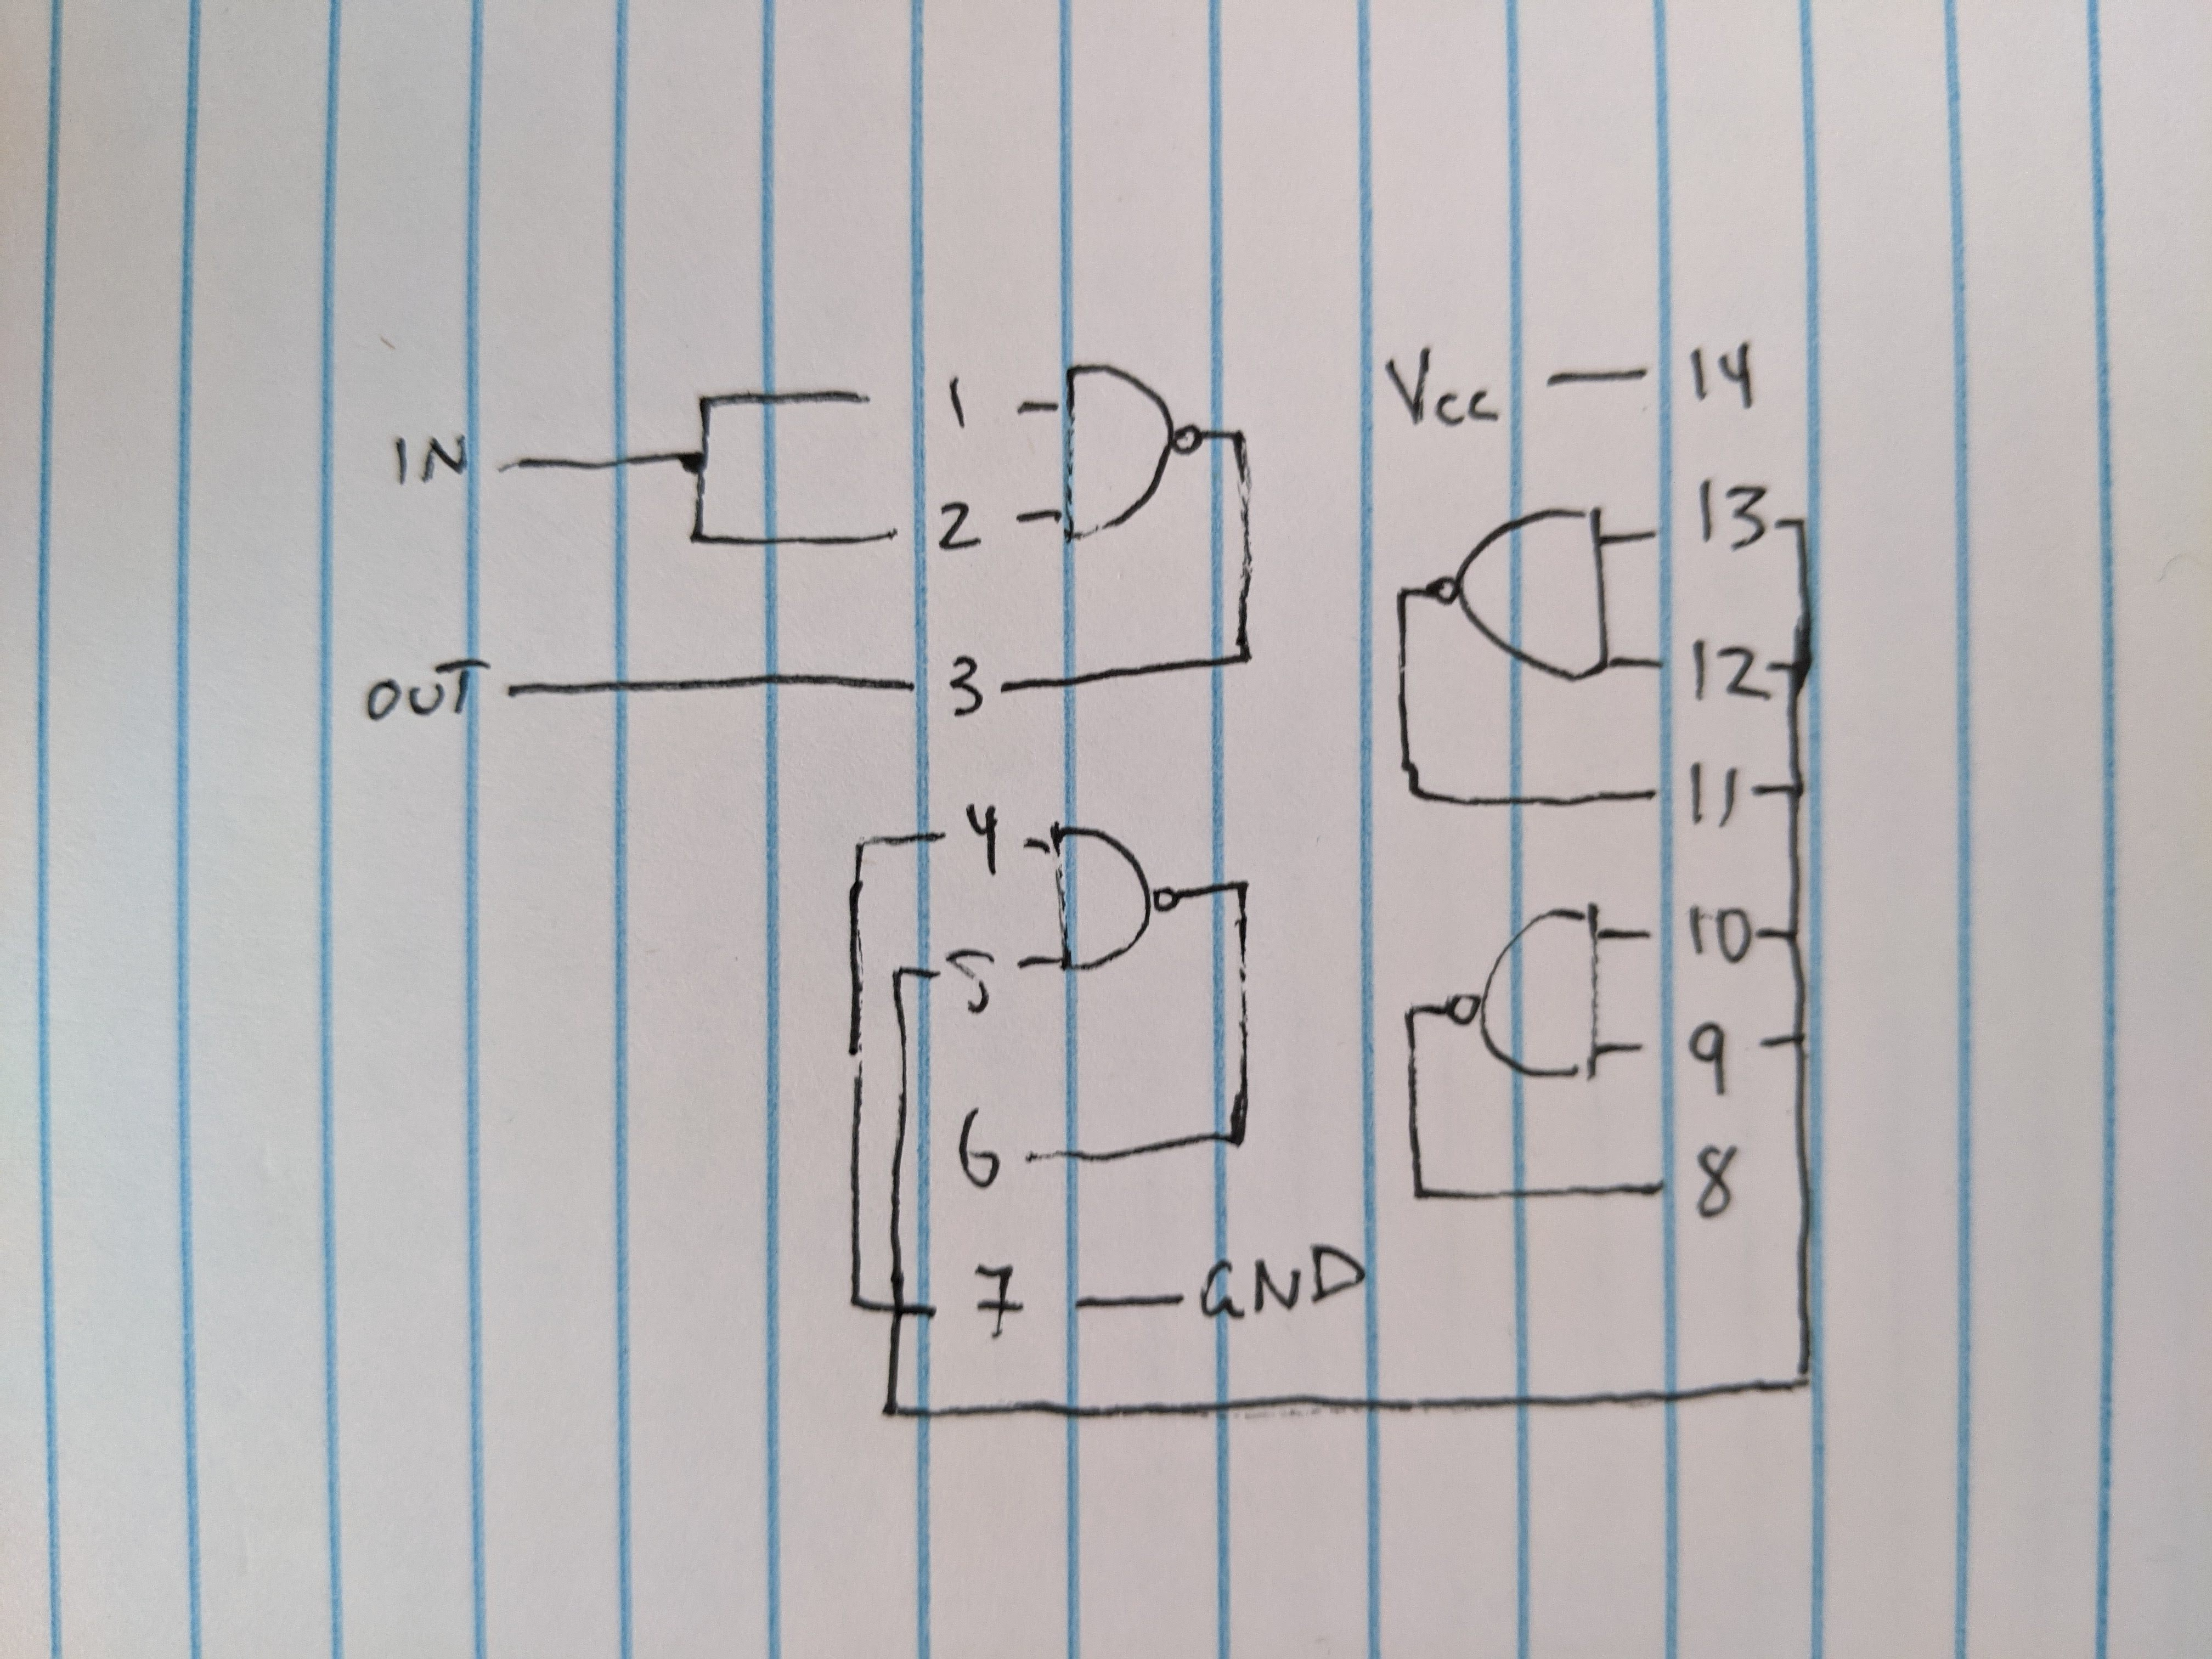
\includegraphics[width=0.7\textwidth]{problem29.jpg}
\end{center}
\problem{0.34} What is the maximum frequency of an ATmega328P when operating
  with $\mathsf{V_{CC}} = 1.8\si{\volt}$? (Consult the datasheet.)

\answer Found in section 29.4.3 Table 29-10 of the ATmega328P datasheet, the maximum frequency is 4\si{\mega\hertz}.

\problem{0.37} Consult a datasheet to find the forward voltage of a red LED
  at 20\si{\milli\ampere}.  If we intend to drive that LED from a
  5\si{\volt} output pin of an ATmega microcontroller, what size E12
  resistor should we use in series with the LED to limit the current to
  20\si{\milli\ampere} or less?  Draw a picture of the circuit.

\answer The datasheet I found had 1.8\si{\volt} as the forward voltage for a red LED. 
We need at least a 90\si{ohm} resistor to limit the LED to 20\si{\milli\ampere}.
\begin{align*}
1.8\si{\volt} = 0.02\si{\ampere} * R\\
R = \frac{1.8\si{\volt}}{0.02\si{\ampere}}\\
R = 90\si{\ohm}
\end{align*}
The closest E12 resistor that guarantees 90\si{\ohm} is a 100\si{\ohm} resistor.
Here is it implemented in a circuit:
\begin{center}
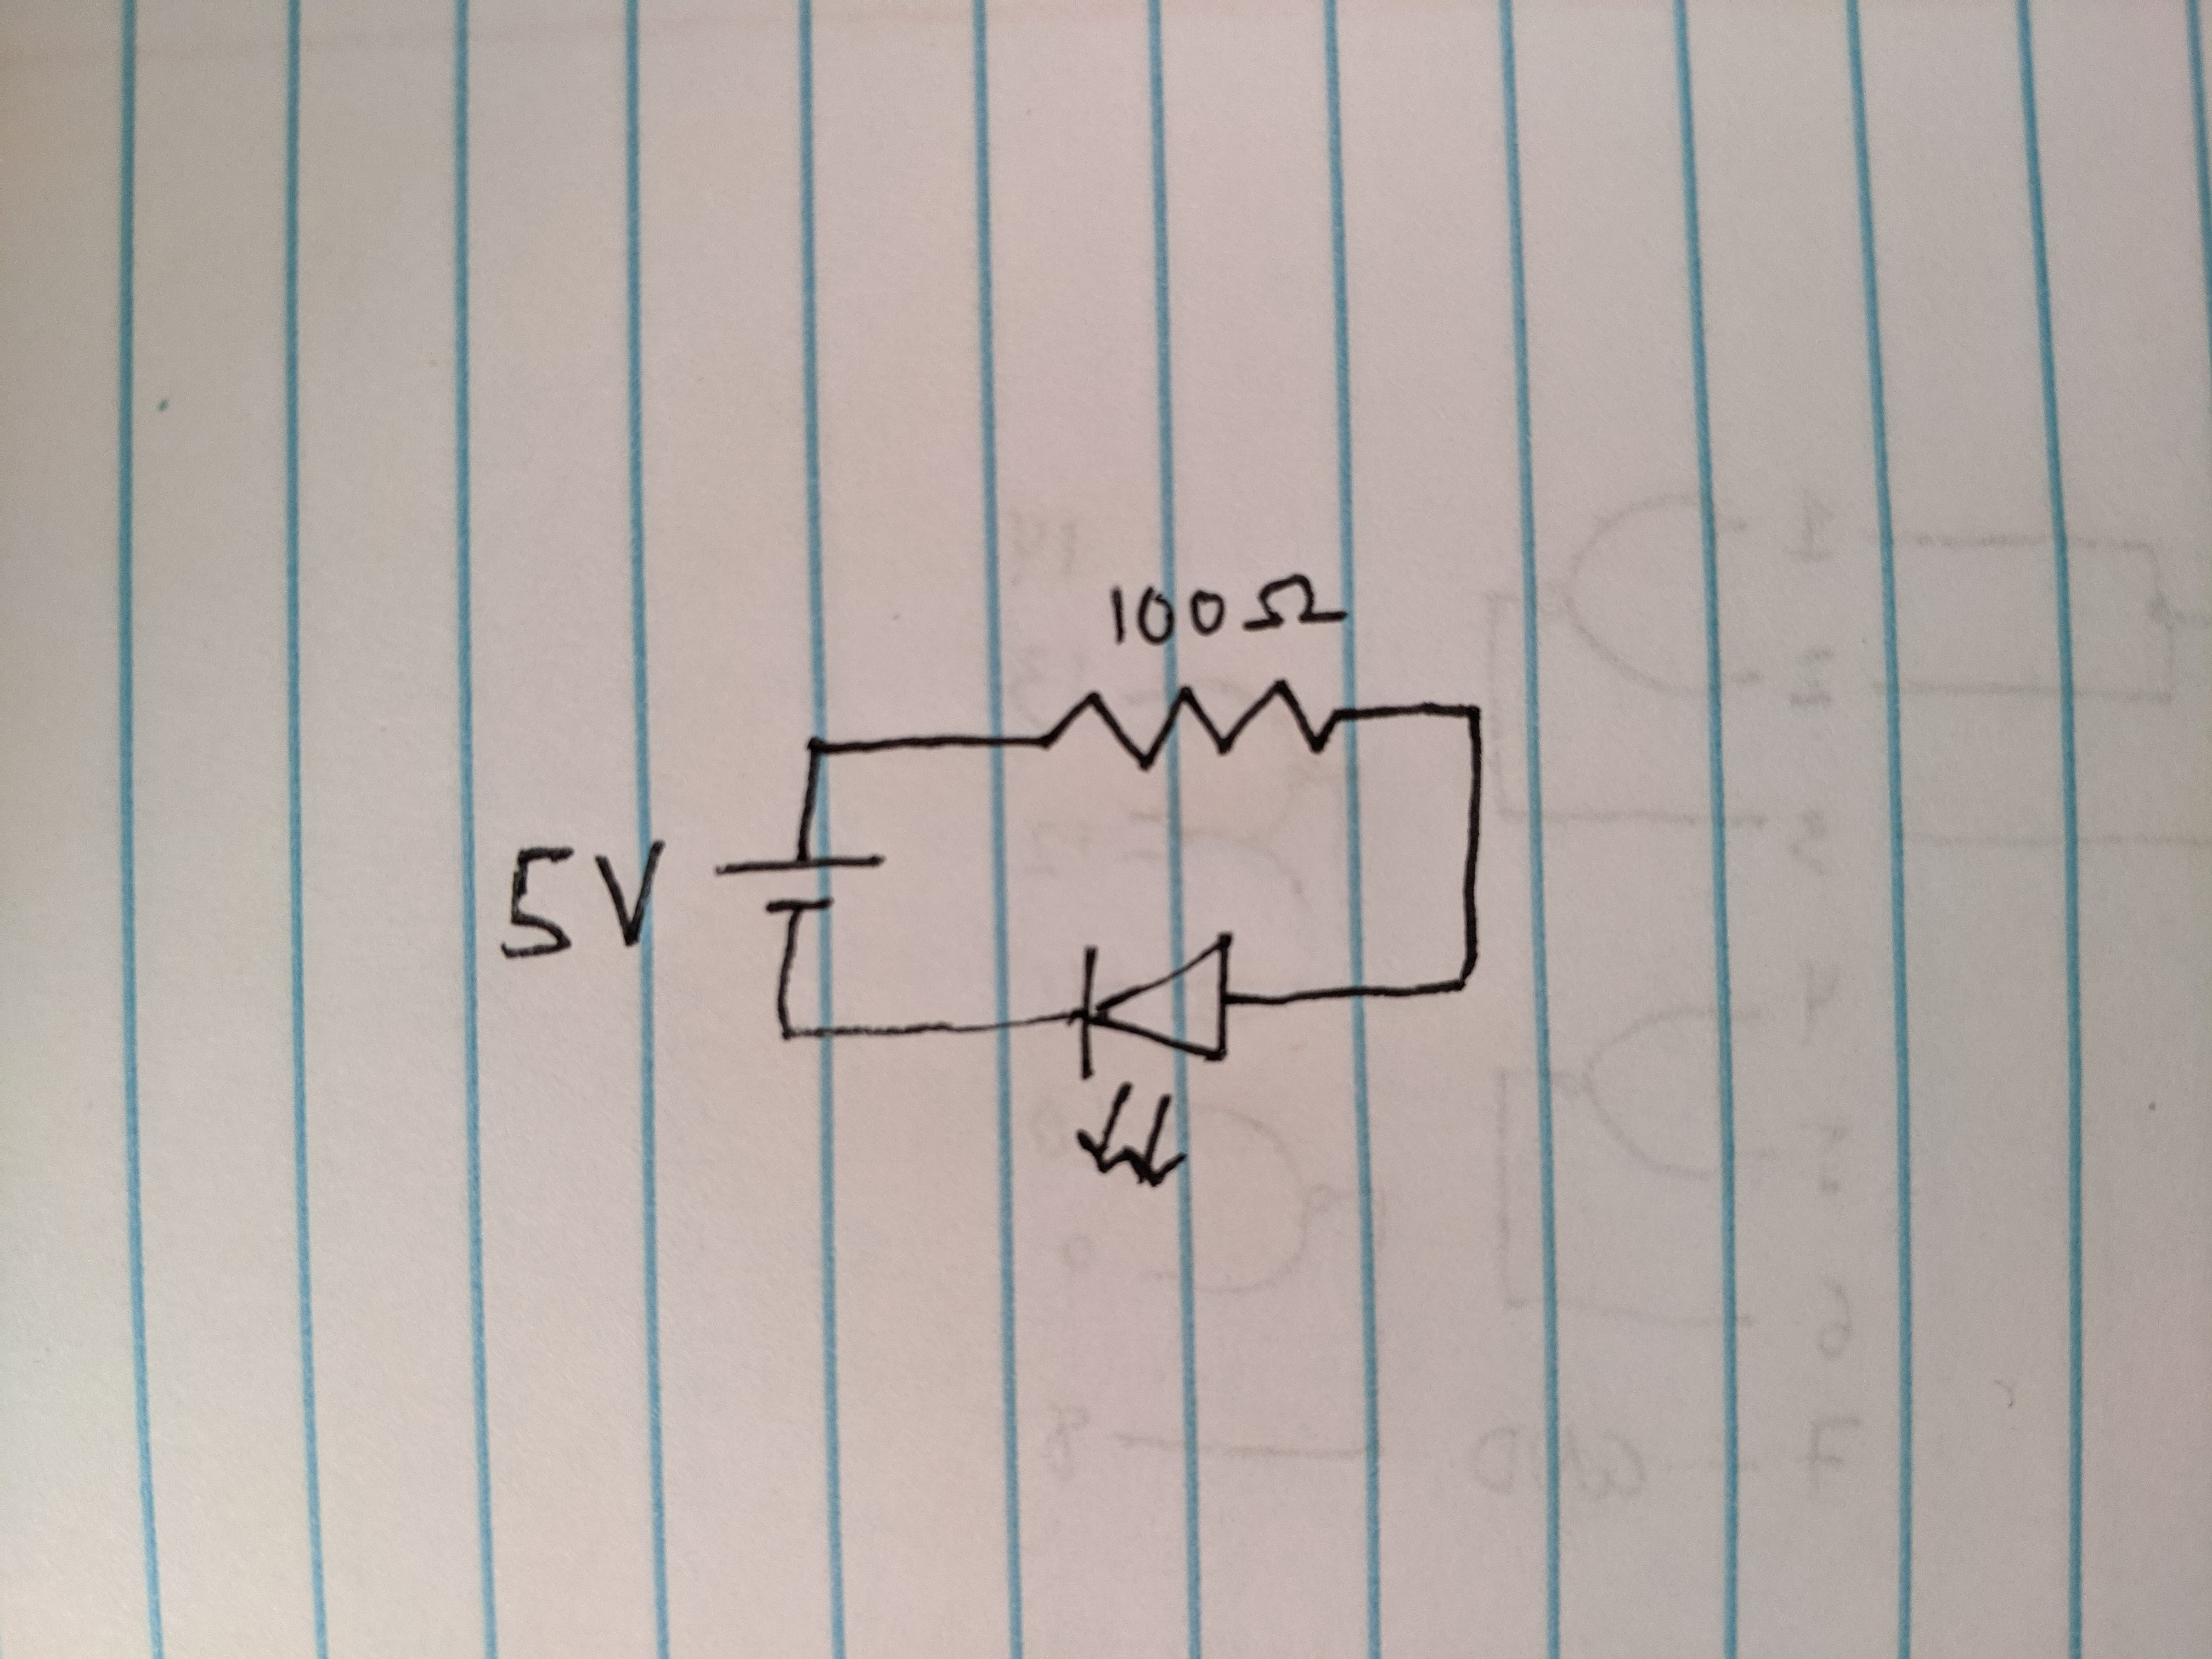
\includegraphics[width=0.7\textwidth]{problem37.jpg}
\end{center}
\end{document}
